\documentclass[11pt,a4paper]{article}

% ---------- Page layout ----------
\usepackage[margin=2.5cm]{geometry}
\usepackage{parskip}            % paragraph spacing instead of indents
\usepackage{microtype}

% ---------- Fonts / maths ----------
\usepackage[T1]{fontenc}
\usepackage{lmodern}
\usepackage{amsmath}
\usepackage{siunitx}            % \SI{6}{\kilo\hertz}
\sisetup{detect-all}

% ---------- Figures (vector only: PDF / PGF / SVG->PDF) ----------
\usepackage{graphicx}
\usepackage{float}
\usepackage[font=small,labelfont=bf]{caption}
\usepackage{subcaption}
\graphicspath{{figures/}}       % save figures from matplotlib as .pdf into ./figures/

% ---------- Tables, links ----------
\usepackage{booktabs}
\usepackage[hidelinks]{hyperref}

% ---------- Code listings for the appendix ----------
\usepackage{xcolor}
\usepackage{listings}
\lstset{
  language=Python,
  basicstyle=\ttfamily\footnotesize,
  keywordstyle=\color{blue!70!black},
  commentstyle=\color{green!40!black},
  stringstyle=\color{orange!70!black},
  numbers=left,
  numberstyle=\tiny\color{gray},
  breaklines=true,
  frame=single,
  columns=fullflexible,
  keepspaces=true,
  showstringspaces=false
}

% ---------- Title info ----------
\title{Digital Signal Processing -- Assignment 1\\
       Fourier Transform: Voice Analysis, Enhancement and Aural Exciter}
\author{
  William Chambers (GUID:\ 2906463C) \\
  Saad Aziz (GUID:\ 2917444A) \\[0.5em]
  University of Glasgow, School of Engineering
}
\date{\today}

\begin{document}
\maketitle

% =====================================================
\section{Recordings}
% =====================================================
% Keep short: just the facts the marker needs.
Voice of one team member, one sentence: ``\textit{Saad and Will are electro wizards.}'' (language: English).
Both recordings are uncompressed WAV, \SI{48}{\kilo\hertz}, 24-bit PCM, mono, not clipped, at distances of \SI{5}{\centi\metre} and \SI{1}{\metre}.

% =====================================================
\section{Task 1: Time and Frequency Analysis (20\%)}
% =====================================================

\subsection{Time and frequency domain plots}
% Method in 2--3 sentences: normalised amplitude vs time; magnitude spectrum in dBFS, % log frequency axis, (1/N) scaling of the FFT.

\begin{figure}[H]
  \centering
  % 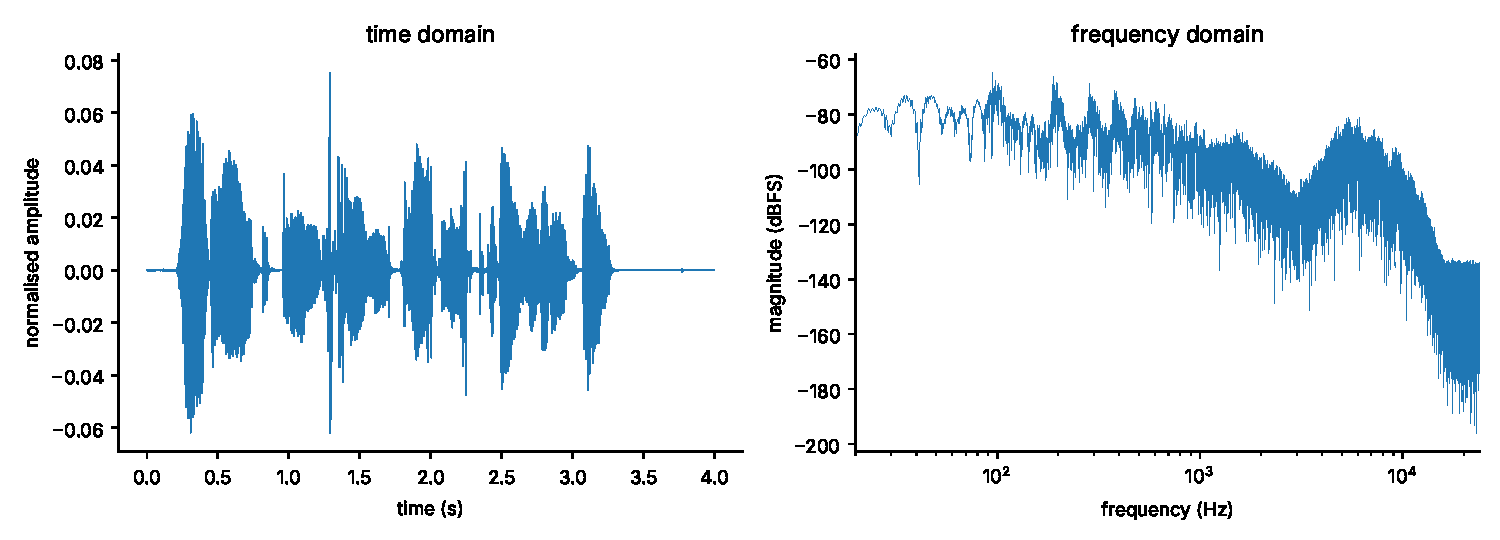
\includegraphics[width=\textwidth]{task1_5cm.pdf}
  \fbox{\parbox{0.9\textwidth}{\centering Placeholder: time + frequency plot, \SI{5}{\centi\metre}}}
  \caption{Voice recorded at \SI{5}{\centi\metre}: (left) time domain, (right) frequency domain.}
  \label{fig:t1_5cm}
\end{figure}

\begin{figure}[H]
  \centering
  % 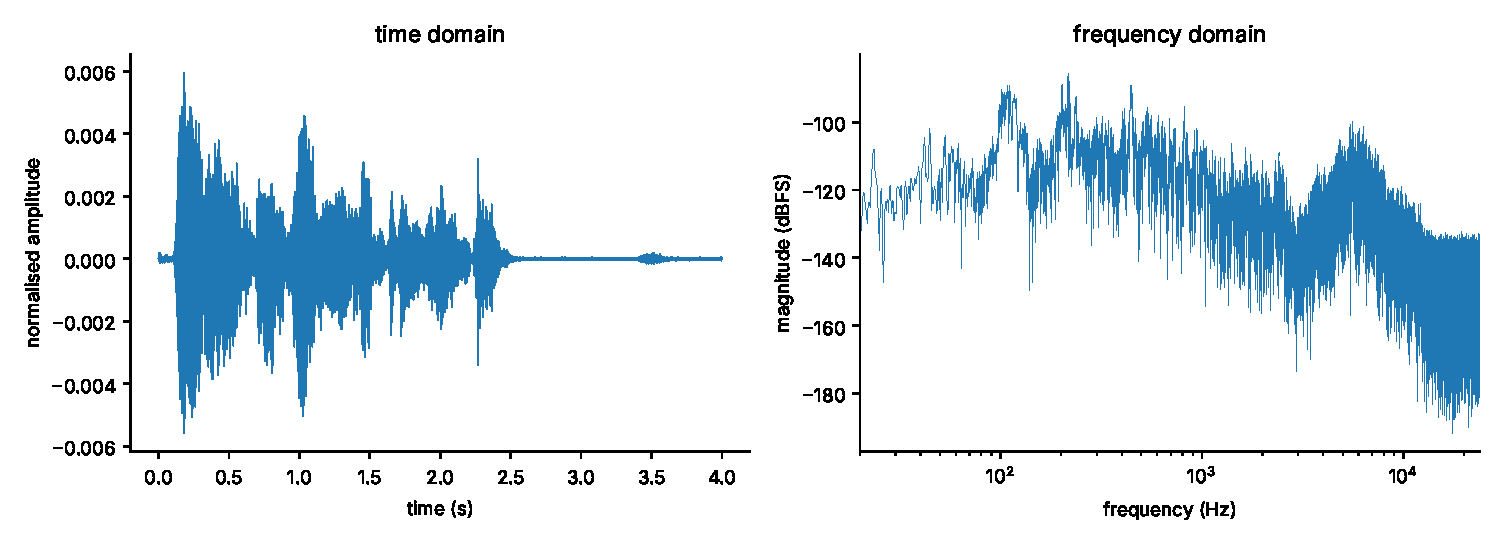
\includegraphics[width=\textwidth]{task1_1m.pdf}
  \fbox{\parbox{0.9\textwidth}{\centering Placeholder: time + frequency plot, \SI{1}{\metre}}}
  \caption{Voice recorded at \SI{1}{\metre}: (left) time domain, (right) frequency domain.}
  \label{fig:t1_1m}
\end{figure}

\subsection{Vowel fundamentals}
% List the chosen peaks per vowel, per recording, and justify (harmonic spacing,
% expected male/female F0 range, harmonic series visible, etc.). No automatic detection.
\begin{table}[H]
  \centering
  \caption{Visually identified vowel fundamentals.}
  \label{tab:vowels}
  \begin{tabular}{lccc}
    \toprule
    Vowel & $f_0$ at \SI{5}{\centi\metre} (Hz) & $f_0$ at \SI{1}{\metre} (Hz) & Justification \\
    \midrule
    /a/ & -- & -- & -- \\
    /e/ & -- & -- & -- \\
    /o/ & -- & -- & -- \\
    \bottomrule
  \end{tabular}
\end{table}

\subsection{Consonant range}
% Range marked up to the highest frequency containing consonant energy + reasoning
% (noise-like broadband energy, e.g.\ 's', 't', 'f' above ...~kHz).

\subsection{Noise region}
% Region that most likely contains only noise + reasoning (flat floor above ... kHz,
% no harmonic structure, level comparable to the silent portions).

\begin{figure}[H]
  \centering
  % 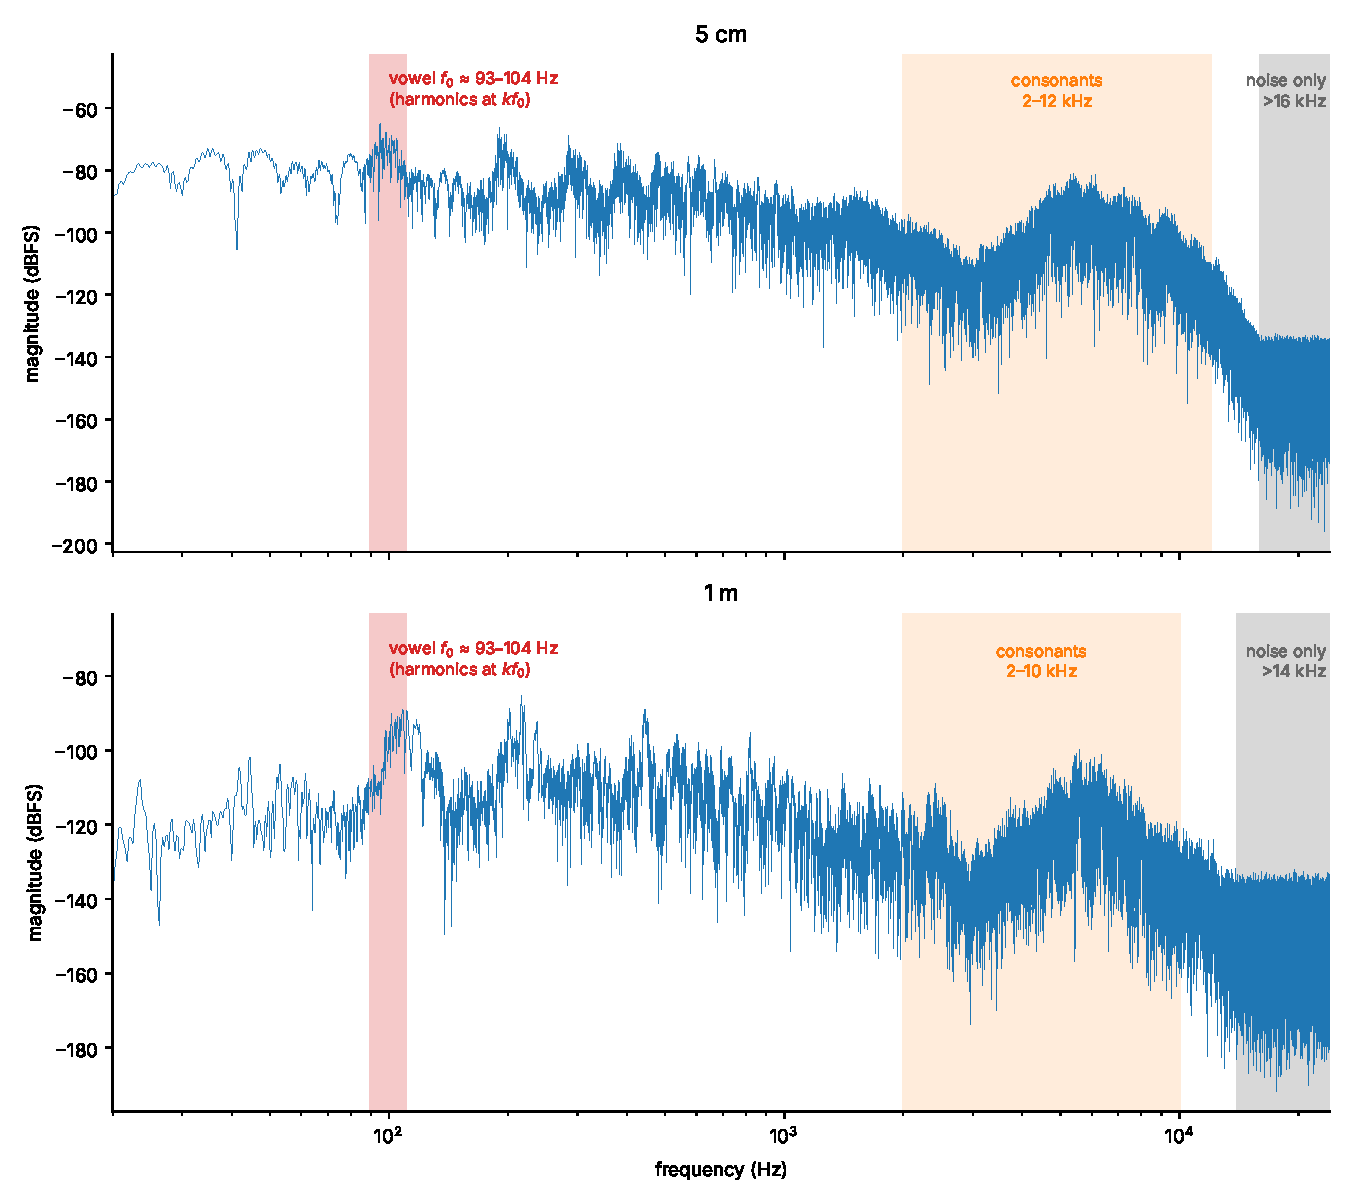
\includegraphics[width=\textwidth]{task1_annotated.pdf}
  \fbox{\parbox{0.9\textwidth}{\centering Placeholder: annotated spectra (vowel peaks, consonant band, noise region)}}
  \caption{Annotated spectra: vowel fundamentals, consonant range and noise-only region.}
  \label{fig:t1_annot}
\end{figure}

% =====================================================
\section{Task 2: Speech Enhancement (20\%)}
% =====================================================

\subsection{Method}
% FFT -> multiply by gain array (dB profile with ramped edges, mirrored for negative
% frequencies so the IFFT is real) -> IFFT -> real part. Mention the scaling to int32 on saving.

\subsection{Noise to be removed}
% For each recording: what kind (room rumble / mains hum / hiss / spike near 500 Hz...)
% and its frequency range.

\subsection{Bass loss with distance and pop sounds}
% 5 cm: proximity effect / plosive energy at low frequencies -> low cut.
% 1 m: bass loss with distance + room effects -> boost around the fundamentals.

\begin{table}[H]
  \centering
  \caption{Gain adjustments applied (final settings).}
  \label{tab:gains}
  \begin{tabular}{lcccl}
    \toprule
    Recording & Band (Hz) & Gain (dB) & Purpose & Reason \\
    \midrule
    5\,cm & 0--60    & -12 & Low cut     & Pops / rumble \\
    5\,cm & 95--400  & +3.5 & Bass boost & Depth \\
    5\,cm & 3000--10000 & +6 & Brightness & Clarity \\
    5\,cm & 12200--Nyq & -12 & High cut   & Hiss \\
    1\,m  & --       & --  & --          & -- \\
    \bottomrule
  \end{tabular}
\end{table}

\begin{figure}[H]
  \centering
  % 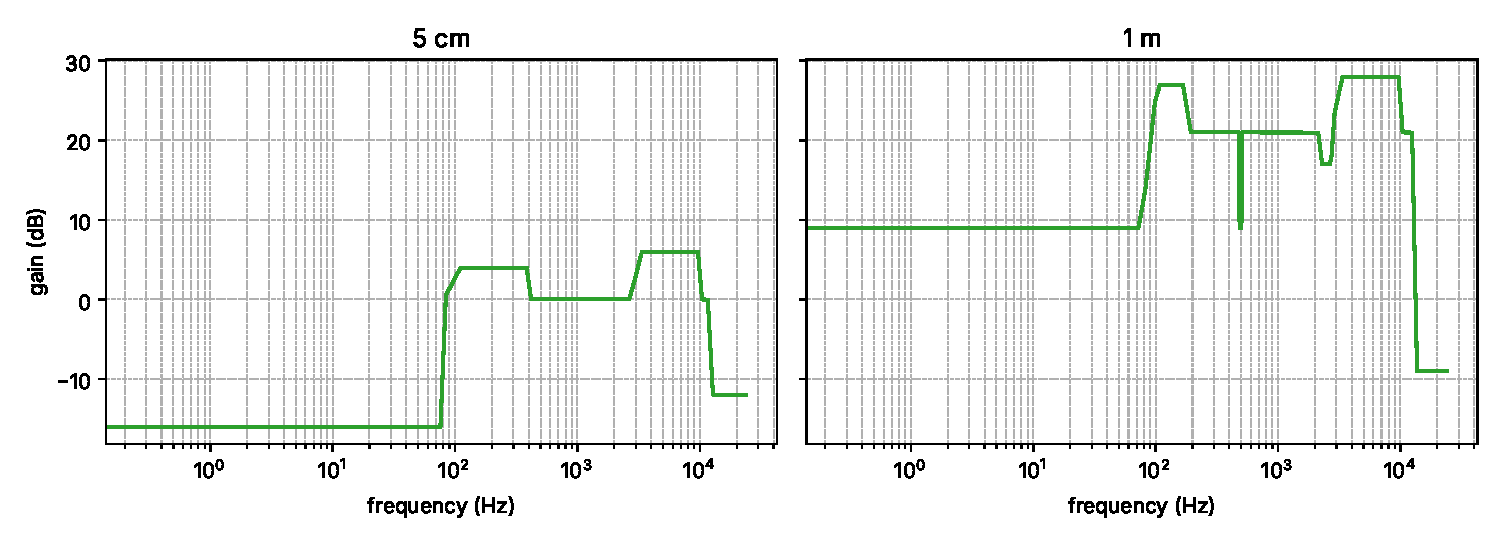
\includegraphics[width=0.9\textwidth]{gain_curves.pdf}
  \fbox{\parbox{0.9\textwidth}{\centering Placeholder: gain curves (5\,cm and 1\,m)}}
  \caption{Gain control curves applied to each recording.}
  \label{fig:gain}
\end{figure}

\begin{figure}[H]
  \centering
  % 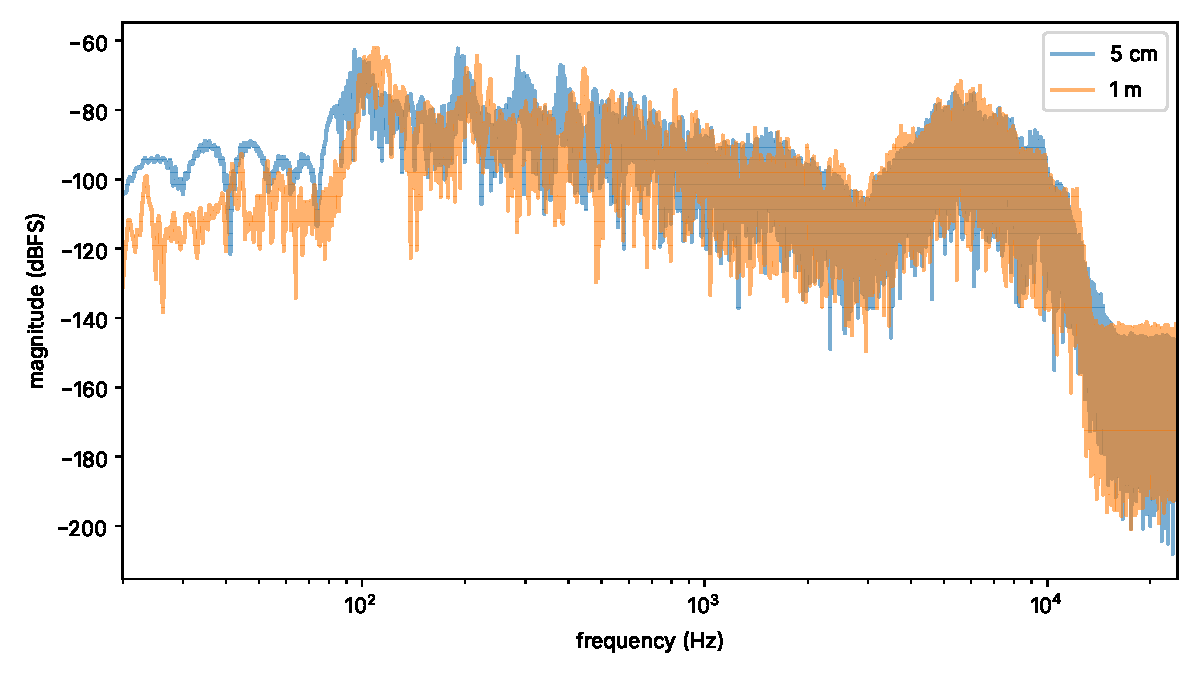
\includegraphics[width=0.9\textwidth]{overlay_enhanced.pdf}
  \fbox{\parbox{0.9\textwidth}{\centering Placeholder: overlay of enhanced 5\,cm vs 1\,m spectra}}
  \caption{Enhanced spectra, \SI{5}{\centi\metre} vs \SI{1}{\metre}.}
  \label{fig:overlay}
\end{figure}

% =====================================================
\section{Task 3: Aural Exciter (60\%)}
% =====================================================

\subsection{Design overview}
% Map your design to the Aphex block diagram: dry path, exciter sidechain
% (band-pass around 2 kHz -> tanh -> pick 3rd harmonic near 6 kHz), optional big-bottom
% sidechain (LPF 50--190 Hz), mixer. Why only a band is fed to the non-linearity and
% why only certain harmonics are kept.
\begin{figure}[H]
  \centering
  % \includegraphics[width=0.9\textwidth]{exciter_block.pdf}
  \fbox{\parbox{0.9\textwidth}{\centering Placeholder: block diagram of your exciter}}
  \caption{Block diagram of the implemented exciter.}
  \label{fig:block}
\end{figure}

\subsection{Pre-processing}
% Pop removal on the 5 cm recording by FFT manipulation (band, gain).

\subsection{Iterative development}
% One subsubsection per iteration: design -> observation -> decision.

\subsubsection{Iteration 1: initial design}
% Parameters: band centre/width, drive, harmonic selection band, mix ratio.
% Result (look at the annotated graph) and what you decided to change.

\subsubsection{Iteration 2: ...}
% What changed and why; observed effect.

\subsubsection{Iteration 3: ...}
% Drive comparison, mix ratio tuning, etc.

\begin{figure}[H]
  \centering
  % 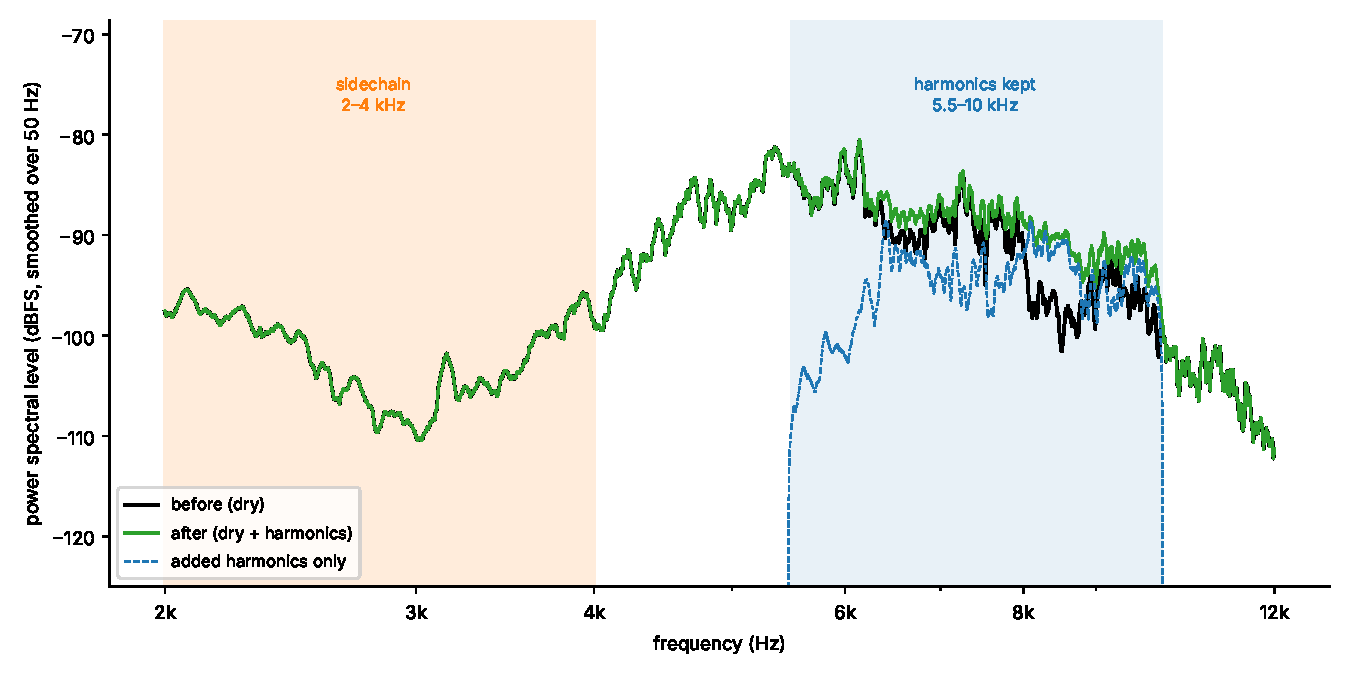
\includegraphics[width=\textwidth]{exciter_before_after.pdf}
  \fbox{\parbox{0.9\textwidth}{\centering Placeholder: annotated spectrum \SIrange{2}{12}{\kilo\hertz}, before vs after}}
  \caption{Annotated spectrum (\SIrange{2}{12}{\kilo\hertz}) before and after the exciter, showing the generated harmonics near \SI{6}{\kilo\hertz}.}
  \label{fig:ba}
\end{figure}

\begin{figure}[H]
  \centering
  % 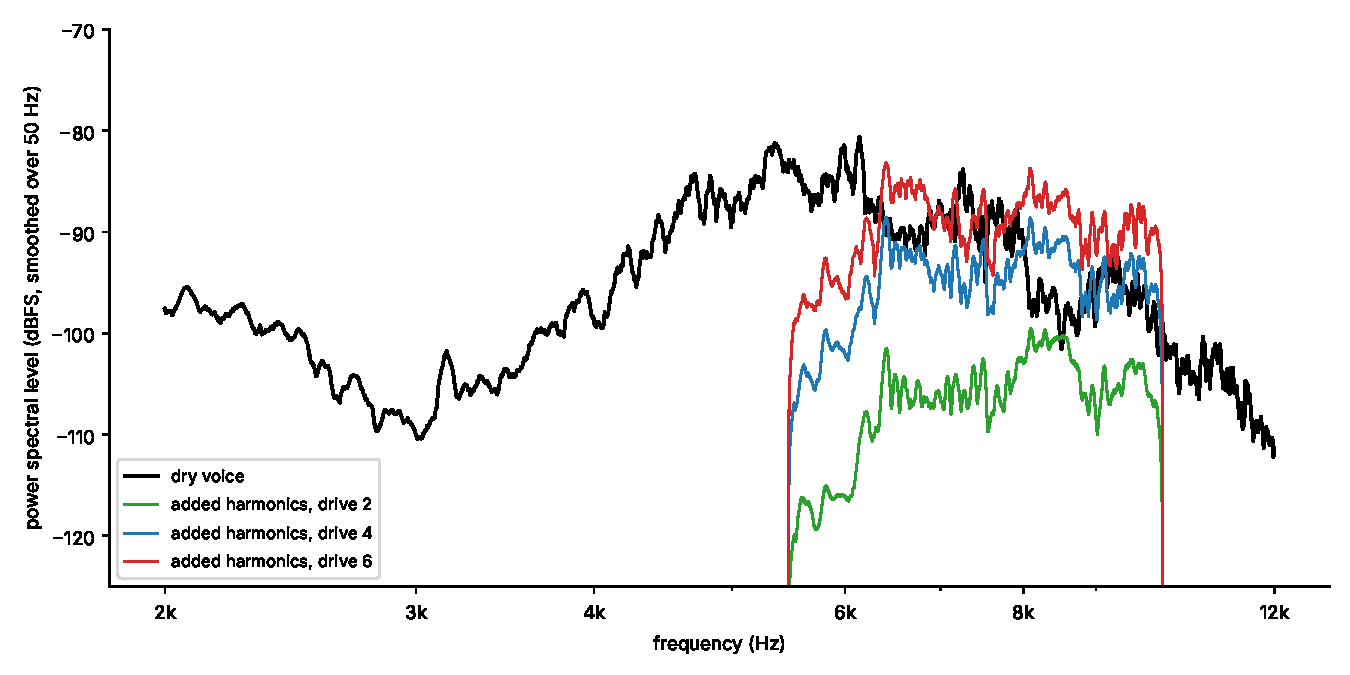
\includegraphics[width=\textwidth]{exciter_drive_compare.pdf}
  \fbox{\parbox{0.9\textwidth}{\centering Placeholder: annotated comparison of drive levels / design changes}}
  \caption{Effect of drive level (or design change) on the harmonic content.}
  \label{fig:drive}
\end{figure}

\subsection{Final design and justification}
\begin{table}[H]
  \centering
  \caption{Final exciter parameters.}
  \label{tab:final}
  \begin{tabular}{ll}
    \toprule
    Parameter & Value \\
    \midrule
    Sidechain band (Hz)            & -- \\
    Non-linearity / drive          & $\tanh$, drive = -- \\
    Harmonic selection band (Hz)   & -- \\
    Mix ratio                      & -- \\
    Big-bottom band (Hz) (if used) & -- \\
    \bottomrule
  \end{tabular}
\end{table}
% Explain why this is the best: spectral evidence, perceived loudness, no unpleasant
% harmonics, amplitude not changed much (e.g.\ compare peak/RMS before and after).

% =====================================================
\section*{Acknowledgement of GenAI Use}
% =====================================================
% Required. State tool name, version, publisher; how it was used; what you did yourself.
\textbf{Tool:} Claude (version: ..., publisher: Anthropic). \\
\textbf{Use:} ... \\
\textbf{Own contribution:} ...

% =====================================================
\appendix
\section{Python Code}
% =====================================================
% Files live next to this .tex file. Update names to match Moodle conventions.

\subsection{run\_tasks.py}
%\lstinputlisting{run_tasks.py}

\subsection{task1\_plot.py}
%\lstinputlisting{task1_plot.py}

\subsection{task2\_enhance.py}
%\lstinputlisting{task2_enhance.py}

\subsection{task3\_exciter.py}
%\lstinputlisting{task3_exciter.py}

\end{document}